\chapter{Introduction and problem statement}
\label{cha:intro}
With the enormous amount of data we produce nowadays, data mining is becoming more and more prevalent.
Consequently, the goal with modern data mining methods is not only to discover information from crude data, but also to condense that information down to concise descriptions and insights.
One such method is redescription mining~\citep{ramakrishnan_turning_2004}.
In a nutshell, it aims to find different ways to describe the same things.

\chapter{Background Knowledge}
\label{cha:background}
In this chapter we are going to explore the underlying theory of the thesis.
We will go from more general knowledge to more specific concepts.
Firstly, the data mining concepts and framework are introduced.
Data mining is the process of extracting information from raw data.
Then we will dig deeper into frequent itemset mining and redescription mining, which are the two main tasks that the thesis is built upon.
\section{Data mining}
\label{sec:datamining}
Why did data mining was developed?
This chapter can give some context about that and then introduces some building blocks of the data mining framework.
\subsection{The problems}
\label{sub:the_problems}
The invention of the computer changed the way we think about storing and managing data.
Unlike books in the library or merchants in the store, data in computers can grow exponentially and instantaneously at a rate like never before.
The need for a systematic way to collect and extract useful information from a big data set started to coin in the late 1980s within companies' research departments \citep{coenen_datamining_2011}.

One of the first problems that data mining tried to solve is to create decision supports from retail clients' transactions and the sales information \citep{coenen_datamining_2011}. 
The aim is to drive the sales up, by giving out suggestions, promotions, and special pricing to the targeted customer based on their behaviors.
For example, retailers can use the system to find out which items are frequently bought together, then arrange them close to each other to create a reminding effect, which can increase the sale.
Advance a few decades later, Netflix - a streaming service company - created a system to recommend movies to users based on their favorites and activities \citep{netflix_rs_2016}.
The most difficult part of such a system is that the data is often significantly smaller than the search space.
An average person can only watch a limited number of movies, while the total number of movies is vastly bigger.
Along with that, nowadays, with the raising of low-cost communicable devices and sensors, we need to find efficient ways to deal with the data produced by them \citep{data_mining_iot_2014}.
Hence, more sophisticated and clever methods are needed; and many have been invented to deal with the growing of the complexities of the problems.

These are just a few examples of some problems that emerged in the modern time of computing and data mining.
As we can imagine, the potential of data mining is unbounded.

\subsection{The main building blocks}
\label{sub:building_blocks}

There are three main phases of data mining: \textit{data collection}, \textit{data wrangling}, and \textit{analytical processing}.

Data collection usually involves the use of hardware or software to acquire raw data.
This could be sensors' data of the environment, or user activities data from computer applications.
The choice of which data to collect is crucial and can affect greatly the quality of the result in the later phases.

After the data is collected, it is usually in a form that is difficult to be processed directly by the algorithms.
That's why we need the data preprocessing phase to make the data easier to be consumed.
This could be structuring the data into known format, e.g. multidimensional formats, time series, etc.; or removing corrupted data.

Analytical processing is the most interesting phase where useful information or insights start to emerge.
From the analytical perspective, we can categorize data mining into four "super problems": clustering, classification, \ac{apm} and outlier analysis \citep{Aggarwal15}.
Even though mining processes are different from each other, they often share some similarities and common patterns that we can generalize and apply similar techniques to them.
For example, association patterns are somewhat similar to overlapping clusters, where each pattern is corresponding to a cluster.

In the scope of this thesis, we will be more interested on the \acl{apm} problem.
\Acl{fim} \citep{borgelt_fim_2012} is the most popular model of \acl{apm}.

% Maybe introduce more type of problems here (Aggarwal15 4.1)

\section{\Acl{fim}}
\label{sec:fim}
\Acl{fim} was originally developed for marketing purposes introduced in \autoref{sub:the_problems}.
The initial goal was to analyze the sale's transactions data to extract information about which items are frequently bought together.
Nowadays, the applications of \acl{fim} expanded to many more domains, with different variety of tasks.

\subsection{Definitions}
Formally, assume that we have a universe of all possible items $\universeOfItemset$.
For example, this can be all the possible products in a groceries store.
Suppose we have a set of $\mathit{n}$ transactions $\transaction{} = \transactionDef{}$, where $\transaction{i}$ is a composition of items from $\universeOfItemset$, with $i$ is the \ac{tid}.
This in turn, could be possible transactions at a groceries store.
Intuitively, we can see that the size of $\universeOfItemset$ is usually much larger than the size of $\transaction{}$: $|\universeOfItemset| \gg |\transaction{} |$.

Such a collection of transactions can be represented in binary representation, where all records have the same length, and each record represents a transaction.
One item in $\universeOfItemset$ will have it own same position in all records.
We can see that the length of each record is basically $|\universeOfItemset|$.
If an item appears in a transaction, it will have value $1$ in the corresponding record, otherwise $0$.
We can see this in the example \autoref{tab:market-basket-dataset}, for the first row, only $Broccoli$ was present in the transaction, hence in the binary representation of the transaction, the first position, which corresponding to $Broccoli$, is set to $1$.
This representation is analogous to a matrix where the rows are the records and represents the transactions, and the columns correspond to the items.
The presence of the $\mathit{j}$th item in the $\mathit{i}$th transaction is determined by the value of the $\mathit{(i, j)}$th entry.

A set of items in $\universeOfItemset$ is an \textit{itemset}. We refer to a set of $k$ items as \kItemset.
The \textit{support} of an itemset is the frequency where it appears in as a subset of a transaction in the dataset.

\begin{definition}[Support \citep{Aggarwal15}]
    The support of an itemset $\itemset$ is defined as the fraction of the transactions in the database $\transaction{} = \transactionDef{}$ that contain $\itemset$ as a subset.
\end{definition}
\begin{sloppypar}
    The support of itemset $\itemset$ is denoted by $\support{I}$.
    For example in \autoref{tab:market-basket-dataset}, $\support{\{Broccoli, Tomato\}} = 0.4$.
\end{sloppypar}
The aim of \acl{fim} is to find the itemsets with supports above a predefined \ac{minsup}.

\begin{definition}[\Acl{fim} \citep{Aggarwal15}]
    Given a set of transactions $\transaction{} = \transactionDef{}$, where each transaction $\transaction{i}$ is a subset of items from $\universeOfItemset$, determine all itemsets $\itemset$ that occur as a subset of at least a predefined fraction $\minsup$ of the transactions in $\transaction{}$.
\end{definition}

\begin{table}[tb]
    \centering
    \begin{tabular}{|l|c|c|}
        \hline
        \textbf{\ac{tid}} & \textbf{Transaction}         & \textbf{Binary representation} \\ \hline
        1            & \{Broccoli\}                 & \texttt{100}                   \\ \hline
        2            & \{Carrot\}                   & \texttt{010}                   \\ \hline
        3            & \{Tomato\}                   & \texttt{001}                   \\ \hline
        4            & \{Broccoli, Tomato\}         & \texttt{101}                   \\ \hline
        5            & \{Broccoli, Tomato, Carrot\} & \texttt{111}                   \\ \hline
    \end{tabular}
    \caption{An example of market basket dataset in binary representation}
    \label{tab:market-basket-dataset}
\end{table}
\subsection{\Acl{arm}}
\label{sub:association_rule_mining}
\Ac{fim} is the first phase of \ac{arm}.
In the following phase, the output of \ac{fim} can be further processed to find the association rules with \acl{arm}.
The result of this step is a set of rules that can be used to predict the behavior of the users.
For example, we can come to a finding that people who buy beer might also buy diapers.
Such strange finding is not quite trivial to thought of, but with the help of \acl{arm}, we can obtain it.

In order to determine whether a rule is trustworthy or not, we need to introduce a new measure: confidence.
The confidence of a rule $X \Rightarrow Y$ is the fraction of transactions containing $X$, which also contain $Y$.
\begin{definition}[Confidence \citep{Aggarwal15}]
    Let $X$ and $Y$ be two set of items.
    The confidence $conf(X \cup Y)$ of the rule $X \cup Y$ is the conditional probability of $X \cup Y$ occurring in a transaction, given that the transaction contains $X$.
    Therefore, the confidence $conf(X \cup Y)$ is defined as follows:
    \begin{equation}
        conf(X \Rightarrow Y) = \frac{sup(X \cup Y)}{sup(X)}
    \end{equation}
\end{definition}
In other words, the confidence of a rule $X \Rightarrow Y$ is the conditional probability that a transaction contains the itemset $Y$, given that it contains the itemset $X$.

For example in \autoref{tab:market-basket-dataset}, the support of $\{Brocoli, Tomato\}$ is $2/5=0.4$, and the support of $\{Broccoli, Tomato, Carrot\}$ is $1/5=0.2$.
Hence, the confidence of the rule $\{Brocoli, Tomato\} \Rightarrow \{Carrot\}$ is $0.2 / 0.4 = 0.5$.

Now since we have the confidence, the definition of an association rule can be presented as follows:
\begin{definition}[Association rules \citep{Aggarwal15}]
    Let $A$ and $B$ be two sets of items.
    The rule $A \Rightarrow B$ is said to be valid at support level $s$ and confidence level $c$, if the following conditions are satisfied:
    \begin{enumerate}
        \item The support of the item set $A$ is at least $s$;
        \item The confidence of $A \Rightarrow B$ is at least $c$;
    \end{enumerate}
    The first criterion ensures that a sufficient number of transactions are relevant to the rule; therefore, it has the required critical mass for it to be considered relevant to the application at hand.
    The second criterion ensures that the rule has sufficient strength in terms of conditional probabilities.
    Thus, the two measures quantify different aspects of the association rule.
\end{definition}
As we can see the confidence together with the minimum support are the core parameters of \acl{arm}.
The minimum support is used in the first phase of \acl{arm} to determine the frequent itemsets.
And the minimum confidence is used in the second phase to determine the association rules.

The frequent itemset mining phase usually takes up most of the computation time of the whole process.
Therefore, most of the research work is focused on it.
\subsection{The \Acl{ne}}
\label{sub:naive_enumeration}
\begin{figure}
    \centering
    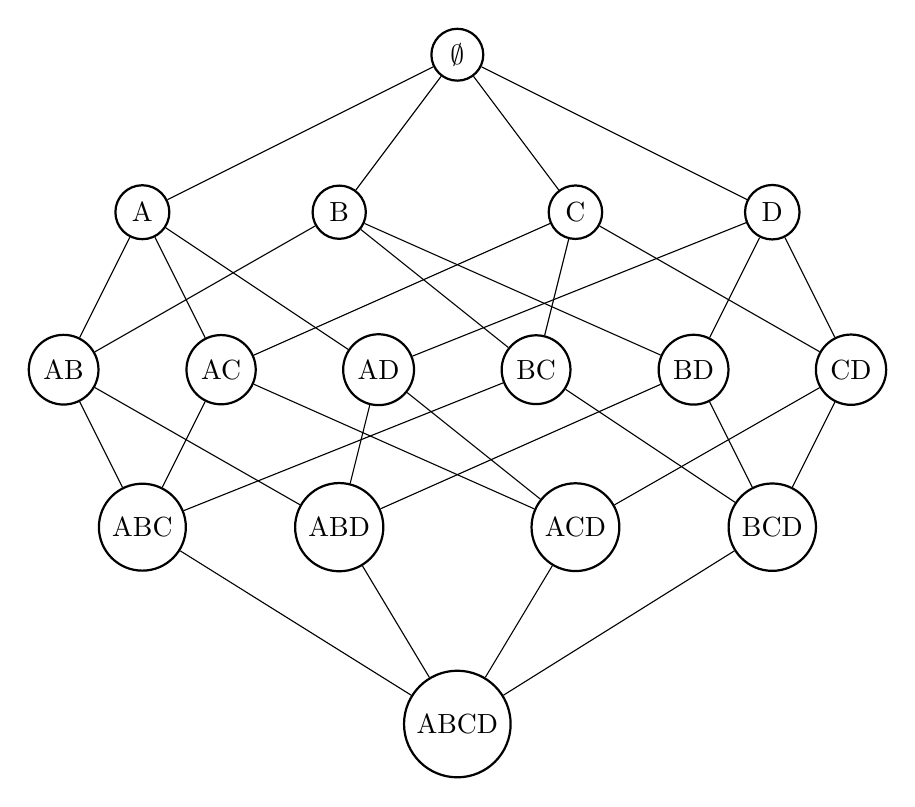
\begin{tikzpicture}[y=-1cm]
        \begin{scope}[every node/.style={circle,thick,draw}]
            \node (E) at (5,0) {$\emptyset$};
            \node (A) at (1,2) {A};
            \node (B) at (3.5,2) {B};
            \node (C) at (6.5,2) {C};
            \node (D) at (9,2) {D};
            \node (AB) at (0,4) {AB};
            \node (AC) at (2,4) {AC};
            \node (AD) at (4,4) {AD};
            \node (BC) at (6,4) {BC};
            \node (BD) at (8,4) {BD};
            \node (CD) at (10,4) {CD};
            \node (ABC) at (1,6) {ABC};
            \node (ABD) at (3.5,6) {ABD};
            \node (ACD) at (6.5,6) {ACD};
            \node (BCD) at (9,6) {BCD};
            \node (ABCD) at (5,8.5) {ABCD};
        \end{scope}
        \draw (E) -- (A);
        \draw (E) -- (B);
        \draw (E) -- (C);
        \draw (E) -- (D);
        \draw (A) -- (AB);
        \draw (A) -- (AC);
        \draw (A) -- (AD);
        \draw (B) -- (AB);
        \draw (B) -- (BC);
        \draw (B) -- (BD);
        \draw (C) -- (AC);
        \draw (C) -- (BC);
        \draw (C) -- (CD);
        \draw (D) -- (AD);
        \draw (D) -- (BD);
        \draw (D) -- (CD);
        \draw (AB) -- (ABC);
        \draw (AB) -- (ABD);
        \draw (AC) -- (ABC);
        \draw (AC) -- (ACD);
        \draw (AD) -- (ABD);
        \draw (AD) -- (ACD);
        \draw (BC) -- (BCD);
        \draw (BC) -- (ABC);
        \draw (BD) -- (ABD);
        \draw (BD) -- (BCD);
        \draw (CD) -- (ACD);
        \draw (CD) -- (BCD);
        \draw (ABC) -- (ABCD);
        \draw (ABD) -- (ABCD);
        \draw (ACD) -- (ABCD);
        \draw (BCD) -- (ABCD);
    \end{tikzpicture}
    \caption{The item lattice for a universe of 4 items.}
    \label{fig:item-lattice}
\end{figure}
Even though the \acl{ne} does not have any practical application, understanding it helps us to understand the computational complexity of \ac{fim} problem and appreciate the benefit of some optimization techniques. %, e.g. pruning or efficient support counting.

The \acl{ne} is, unsurprisingly, very simple. It tries to check all the possible combinations to see if one is a frequent itemset or not.
For example, with the universe of 4 items, all the possible combinations of items are represented in \autoref{fig:item-lattice}.
In order to check the frequency of an itemset, we need to count the number of transactions that contain the itemset, this step is called \textit{support counting}.

Considering a universe of items $\universeOfItemset$, there will be a total of $2^{\left\lvert \universeOfItemset \right\rvert} - 1$ possible combinations, or itemsets, excluding the empty set.
In other words, the size of the possible itemsets grows exponentially with the size of the universe.
To put this into perspective, a universe of 100 items will have a total of $2^{100} - 1$ possible itemsets, which is bigger than $10^{30}$.
At the time of writing this, the most powerful supercomputer is the Fugaku with the speed of approximately 0.4 exaflop/s \citep{monroe_fugaku_2020}.
Suppose we use this supercomputer to enumerate through the search space of all $10^{30}$ possible itemsets, this will take at least $2.5^{12}$ seconds, or at least 79 thousands years.
And all that was just for enumerating the search space, we are supposed to do the support counting at each stop and that will take much more time than the enumeration.
Realistically, the size of $\universeOfItemset$ is often much bigger than 100.
To say the least, the \acl{ne} is not practical, even for datasets over small collections of items.
Let's see how can we improve this with some optimization techniques in the following subsection.

% We will discuss some properties that can be used to optimize the frequent itemset mining phase in \autoref{sub:optimization_techniques }.
\subsection{The \acl{apriori}}
\label{sub:optimization_techniques}
As described in \autoref{sub:naive_enumeration}, \acl{fim} often involves iterating through a large dataset and huge search space.

In the \acl{ne}, a lot of candidates are generated by the algorithm for each iteration.
Thus, a sensible approach is to reduce the search space by pruning some candidates, or better not generating those that we know they will not be frequent.
We know that if an itemset $I$ exists in a transaction, then all of its subsets $J_1, J_2, \dots, J_k$ must also exist in the transaction.
Hence, the number of transactions that one subset $J_i$ can be found in is always larger or equal to the corresponding value of the itemset $I$. This is called the \acl{smp}:
\begin{definition}[\Acl{smp} \citep{Aggarwal15}]
    The support of every subset $J$ of $I$ is at least equal to that of the support of itemset $I$.
    \begin{equation}
        sup(J) \geq sup(I) \quad \forall J \subseteq I
    \end{equation}
\end{definition}

The direct implication from the \acl{smp} is that every subset $J_i$ of a frequent itemset $I$ is also frequent.
This is also called the \acl{dcp} \citep{Aggarwal15}.
We can apply this property in the opposite direction, that is, if a subset $I$ is not frequent, then all of its supersets $J_1, J_2, \dots, J_k$ must not be frequent.
For example in the \autoref{fig:item-lattice}, if during the searching, we found out that $I = \{A, B\}$ is not frequent, then all the supersets of $I$, e.g. $\{A, B, C\}, \{A, B , D\}, \{A, B , C, D\}$, cannot be frequent.
We can then drop all supersets of ${I = \{A, B\}}$ from the search space.
This is a huge advantage since it allows us to stop searching branches early if we know that one of the subsets is not frequent.
What we have here is essentially the core of the \acl{apriori}, where the \acl{dcp} is applied to a \ac{ne}.
By utilizing the simple \acl{dcp} property above, the amount of candidates we have to process is drastically reduced.

However, for each candidate, we still have to count the support of it, which itself is usually a very expensive task if done naively.
Trying to count the support more efficiently is also a good way to improve the performance.
One method is to prune the transactions that irrelevant to the candidate.
In \citep{brin_et_al_1997}, the \ac{dic} algorithm was presented, where itemsets are dynamically added and deleted as transactions are read.

% TODO: develop more on Apriori optimization techniques.
% Of course there are more techniques that can be applied to improve the \acl{apriori}.
% A more advanced technique is to use some data structure to store the candidates and/or transactions in a way that can be used to count the support efficiently.

% For instance, in \citep{bodon2003fast}, a Trie data structure was used store the candidates so that we can quickly retrieve the supports of an itemset, and generate the candidates faster.

\subsection{ECLAT}
The family of algorithms that enumerate the search space horizontally with increasing size of the candidates are called the \acl{lwa}.
There are also approaches where the algorithms traverse the search space vertically

\section{Redescription mining}


\chapter{Employing ECLAT for Redescription Mining}
\label{cha:employment}

\chapter{Experiments}
\label{cha:experiments}

\chapter{Conclusions}
\label{cha:conclusions}